\documentclass[dvipsnames,crop=true]{standalone}
\usepackage{tikz}
\usetikzlibrary{calc,external,positioning}
\usepackage{amsmath}
\begin{document}

  \tikzsetnextfilename{simpl_geom}
  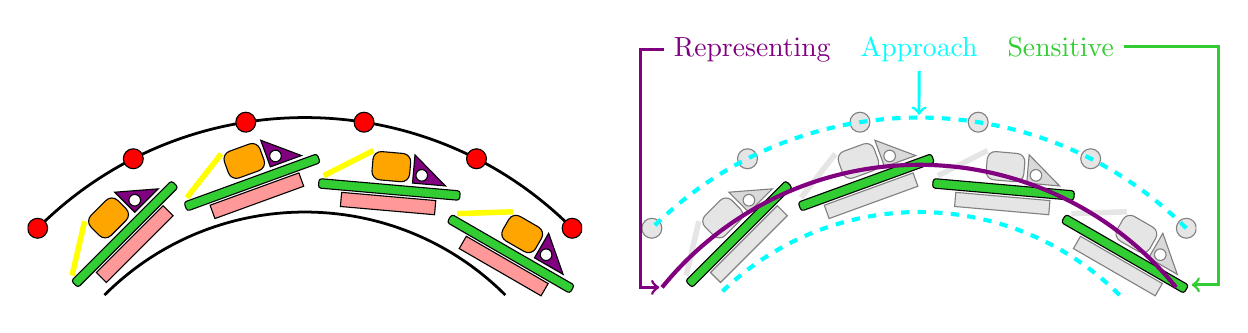
\begin{tikzpicture}[scale=0.6]
    \def\ao{90}
    \def\as{45}
    \pgfmathsetmacro{\al}{-\as+\ao}
    \pgfmathsetmacro{\ar}{\as+\ao}
    \def\ri{6}
    \def\ro{8}
    \pgfmathsetmacro{\rm}{(\ro+\ri)/2}

    \newcommand{\dbox}[4]{
      \def\w{#2}
      \def\h{#3}
      \node[#4,inner sep=0,minimum width=\w,minimum height=\h] (#1) at (0,0) {};
    }
    \def\n{5}

    \begin{scope}[shift={(-6.5  ,0)}]
      \coordinate (bl) at ({-cos(\al)*\ro}, {sin(\al)*\ri});
      \coordinate (tr) at ({cos(\al)*\ro}, \ro);
      \coordinate (pad) at (6pt,6pt);
      \clip ($(bl) - (pad)$) rectangle ($(tr) + (pad)$);

      \foreach \r in {\ri,\ro} {
        \draw[line width=1pt] (0,0) ++ (\al:\r) arc (\al:\ar:\r);
      }

      \foreach \i in {0,...,\n} {
        \pgfmathsetmacro{\a}{\al + (\ar-\al)/\n * \i}
        \draw[fill=Red] (\a:\ro) circle(6pt);
      }


      \foreach \i in {0,...,3} {
        \pgfmathsetmacro{\ma}{-\as + \i*25 + 5}
        \begin{scope}[rotate=\ma,transform shape]
          \begin{scope}[transform shape,shift={(0,\rm)},rotate=10]
            \begin{scope}[shift={(0,0.2)}]
              \dbox{b1}{8mm}{6mm}{draw,fill=Orange,rounded corners=3pt}
            \end{scope}
            \begin{scope}[shift={($(b1.south) + (0,-2pt)$)}]
              \dbox{b2}{3cm}{2mm}{draw,anchor=north,fill=LimeGreen,rounded corners=1pt}
            \end{scope}
            \begin{scope}[shift={($(b2.south) + (0,-1pt)$)}]
              \dbox{b3}{2cm}{3mm}{draw,anchor=north,fill=Red!40}
            \end{scope}

            \begin{scope}[shift={($(b1.south east) + (2pt,0pt)$)}]
              \draw[fill=Purple] (0,0) --(7mm,0) --(0,6mm) -- cycle;
              \draw[fill=white] (1.8mm,1.8mm) circle(3.5pt);
            \end{scope}
            \draw[line width=2pt,shorten >=2pt,Yellow] (b1.north west) -- (b2.north west);
          \end{scope}
        \end{scope}
      }

    \end{scope}

    \def\thec{Black!10}
    
    \begin{scope}[shift={(6.5,0)},draw=Black!50]
      \coordinate (bl) at ({-cos(\al)*\ro}, {sin(\al)*\ri});
      \coordinate (tr) at ({cos(\al)*\ro}, \ro);
      \coordinate (pad) at (6pt,6pt);
      \clip ($(bl) - (pad)$) rectangle ($(tr) + (pad)$);

      \foreach \i in {0,...,\n} {
        \pgfmathsetmacro{\a}{\al + (\ar-\al)/\n * \i}
        \draw[fill=\thec] (\a:\ro) circle(6pt);
      }
      
      \foreach \r in {\ri,\ro} {
        \draw[line width=1.5pt,Cyan,dashed] (0,0) ++ (\al:\r) arc (\al:\ar:\r);
      }

      \coordinate (appo) at (90:\ro);

      \foreach \i in {0,...,3} {
        \pgfmathsetmacro{\ma}{-\as + \i*25 + 5}
        \begin{scope}[rotate=\ma,transform shape]
          \begin{scope}[transform shape,shift={(0,\rm)},rotate=10]
            \begin{scope}[shift={(0,0.2)}]
              \dbox{b1}{8mm}{6mm}{draw,fill=\thec,rounded corners=3pt}
            \end{scope}
            \begin{scope}[shift={($(b1.south) + (0,-2pt)$)}]
              \dbox{b2}{3cm}{2mm}{draw,anchor=north,fill=LimeGreen,draw=Black,rounded corners=1pt}
              \coordinate (sepo\i) at (15mm,0);
            \end{scope}
            \begin{scope}[shift={($(b2.south) + (0,-1pt)$)}]
              \dbox{b3}{2cm}{3mm}{draw,anchor=north,fill=\thec}
            \end{scope}

            \begin{scope}[shift={($(b1.south east) + (2pt,0pt)$)}]
              \draw[fill=Black!15] (0,0) --(7mm,0) --(0,6mm) -- cycle;
              \draw[fill=white] (1.8mm,1.8mm) circle(3.5pt);
            \end{scope}
            \draw[line width=2pt,shorten >=2pt,\thec] (b1.north west) -- (b2.north west);
          \end{scope}
        \end{scope}
      }
      
      \def\aext{6}
      \draw[line width=1.5pt,Purple] (0,0) ++ ({\al-\aext}:\rm) arc ({\al-\aext}:{\ar+\aext}:\rm) coordinate[at end] (repo);

      \coordinate (label) at (0,{\ro + 1.3});

    \end{scope}

    \node[Cyan,anchor=base] (alabel) at (label) {Approach};
    \node[Purple,left=of label,anchor=base east] (rlabel) {Representing};
    \node[LimeGreen,right=of label,anchor=base west] (slabel) {Sensitive};

    \begin{scope}[line width=1pt,shorten >=1pt]
      \draw[->,Cyan] (alabel) -- (appo);
      \draw[->,Purple] (rlabel.west) --++(-0.5cm,0) |- (repo);
      \draw[->,LimeGreen] (slabel.east) --++(2cm,0) |- (sepo0);
    \end{scope}

    \coordinate (ml) at (0, {(\ro + sin(\al)*\ri)/2});
    % \fill (ml) circle(2pt);
    % \draw[->,line width=2pt] (ml) ++(-1,0) -- ++(2,0);

  \end{tikzpicture}

\end{document}